\section{РУКОВОДСТВО ПОЛЬЗОВАТЕЛЯ}
\label{sec:manual}

В данном разделе описана информация, которая необходима пользователям
разрабатываемой системы для ее корректного использования.

Поскольку данный дипломный проект является библиотекой, у него будет
несколько групп пользователей:
\begin{itemize}
    \item разработчики, которые будут ее использовать при создании собственных продуктов;
    \item пользователи разработанных продуктов.
\end{itemize}

Поскольку у продукта отсутствует визуальный интерфейс и другие способы
взаимодействия с системой, которые не могут быть уточнены или переопределены,
дальнейшее описание касается в первую очередь тех людей, кто будет
производить разработку и отладку результирующего продукта, составной частью которого
является текущая библиотека.

\subsection{Общее описание особенностей}

Разрабатываемая в контексте данного дипломного проекта
часть системы поставляется в виде исходных кодов и способна работать
на операционных системах реального времени, таких как FreeRTOS и TI-RTOS, так и
на настольных и серверных операционных системах, таких как Linux.

Для дальнейшего удобства использования система разбита на несколько пакетов:
платформозависимый OSAL и платформонезависимые OsalApi, Shared, libiec61850,
libxml2, GooseReceiver.
В случае необходимости добавления поддержки новой операционной системы разработчик
должен создать аналог библиотеки OSAL, в которой он реализует все программные
интерфейсы для доступам к примитивам синхронизации, а также остальные составляющие
модуля \moduleOsal.

Пакет OsalApi отличается от других пакетов, поскольку
является интерфейсным и содержит только набор заголовочных файлов
с описание прототипов функций модуля \moduleOsal.
Из-за отсутствия файлов с исходным кодом
сборка этого пакета не зависит от используемых компиляторов и целевых архитектур.

\nomenclaturex{OSAL}{Operating System Abstraction Layer}{уровень абстракции операционной системы}

В случае, если разработчику будет необходимо добавить поддержку новой архитектуры
или компилятора, ему будет необходимо добавить их поддержку в систему сборки
и скомпилировать все поставляемые пакеты с созданными настройками, кроме OsalApi.

\subsection{Требования к аппаратному и программному обеспечению}

Для сборки и дальнейшего использования данного дипломного проекта необходимо
следующее программное обеспечение:
\begin{itemize}
    \item операционная система на основе ядра Linux, на котором будет производится сборка пакетов;
    \item среда исполнения языка программирования Python версии 3.6 или новее для вызова пакетного менеджера с необходимыми параметрами;
    \item пакетный менеджер Conan версии 1.48.0 или новее для создания необходимых пакетов;
    \item кроссплатформенная система сборки CMake версии 3.20.0 или новее
    для автоматизации сборки целевого проекта;
    \item основная система сборки Make версии не ниже 4.0 для выполнения всех команд,
    сгенерированных CMake;
    \item среда исполнения языка программирования Ruby версии не ниже 2.3.0
    для генерации вспомогательных файлов тестирования пакета;
    \item компилятор для языка C с поддержкой стандарта C99 для создания объектных
    файлов из исходных кодов;
    \item утилита архивации, которая поддерживается целевым компоновщиком,
    предназначенная для создания единого архива объектных файлов для каждого пакета.
\end{itemize}

\subsubsection{Целевая операционная система Linux}

Для обеспечения сборки исходных кодов пакета OSAL также необходима поддержка
C++11, поскольку часть реализаций платформозависимых компонентов используют
этот язык.

Для компиляции и связывания исходных кодов используется используется
набор инструментов GCC версии 9.3.0 или новее с целевой архитектурой amd64.
В него входят компиляторы \lstinline{gcc} и \lstinline{g++} для языков C и C++ соответственно,
утилита архивации \lstinline{ar},
компоновщик \lstinline{ld} и другие компоненты, обеспечивающие дополнительный набор функций.

\nomenclaturex{GCC}{GNU Compiler Collection}{набор компиляторов GNU}

\subsubsection{Целевая операционная система FreeRTOS}

Операционная система FreeRTOS является операционной системой реального времени
и по умолчанию представлена монолитной структурой без поддержки файловых систем.
Поэтому для получения объектных файлов используется кросс-компиляция
с помощью набора инструментов GCC версии 7.3.1. Целевой архитектурой
является ARM.

\nomenclaturex{ARM}{Advanced RISC Machine}{усовершенствованная RISC-машина}

В качестве примера использования этой операционной системы взята отладочная плата
STM32H745I-DISCO, следовательно для программирования и отладки кода рекомендуется использовать
среду разработки STM32CubeIde версии 1.4.0 или новее. В указанной версии
содержится используемый для сборки набор инструментов.

\subsubsection{Целевая операционная система TI-RTOS}

Операционная система TI-RTOS похожа по своим концепциям на FreeRTOS, поэтому
имеет те же особенности с используемыми наборами инструментов.

Для отладки платформозависимого кода используется отладочная плата TMDSIDK572
под управлением процессора AM5728 с архитектурами ARM и C66x, поэтому
содержит различные утилиты сборки.
Необходимые наборы инструментов для сборки исходных кодов поставляются
в TI-RTOS SDK для процессоров Sitara AM57xx компании Texas Instruments версии
06.03.00.106. Для отладки рекомендуется использовать фирменную среду разработки
Code Composer Studio версии 11.1.0 или новее.

\nomenclaturex{SDK}{Software Development Kit}{комплект для разработки программного обеспечения}

\subsection{Настройка рабочего окружения}

Основной платформой, которая заявлена в требованиях,
является операционная система семейства Linux.
В качестве примера, на котором будет показана установка всех необходимых
зависимостей, была взята Ubuntu 22.04 LTS amd64 как самая свежая версия одного из самых популярных дистрибутивов на момент написания текущего руководства.

\nomenclaturex{LTS}{Long-Term Support}{увеличенный срок поддержки}

Порядок установки выбранной операционной системы описан в
источнике~\cite{ubuntu_how_to_install}. Несмотря на то, что там расписан порядок
установки для более старой версии данного дистрибутива, выбранный вариант
полностью соответствует новой версии.
Скачать необходимую версию дистрибутива можно с официального
сайта~\cite{ubuntu_download_site}.

После установки операционной системы необходимо установить программное
обеспечение, поставляемое в качестве ее компонентов. Сделать это можно из
терминала с помощью следующих команд:

\begin{lstlisting}
$ sudo apt update
$ sudo apt install -y python3 python3-pip cmake make ruby gcc g++
$ pip3 install conan
\end{lstlisting}

Указанные команды установят все необходимые для запуска сборки зависимости.
Для корректной работы утилит рекомендуется перезапустить терминал или весь
персональный компьютер, иначе утилита \lstinline{conan} может быть недоступна.

Установка сред разработки для целевых платформ FreeRTOS и TI-RTOS
описана в официальной документации~\cite{st_cubeide_install}
и~\cite{ti_ccs_install} соответственно.
Порядок установки TI-RTOS SDK для семейства AM57xx также
предоставлен его разработчиками~\cite{ti_sdk_install}.

\subsection{Сборка исходных кодов}

Для сборки разработанной библиотеки необходимо скопировать ее с диска, поставляемого
с дипломным проектом, на компьютер. Сделать это можно как средствами
графического интерфейса, так и с помощью утилит командной строки.

Поставляемые пакеты необходимо собирать в следующем порядке для корректного
разрешения зависимостей:
\begin{enumerate_num}
    \item OsalApi.
    \item Shared.
    \item OSAL для операционной системы Linux.
    \item libiec61850.
    \item libxml2.
    \item GooseReceiver.
\end{enumerate_num}

Сборка пакетов в ином порядке может привести к получению ошибок
отсутствия зависимостей или использованию их старых версий.
Поскольку сборка каждого компонента выполняется идентично, она будет
продемонстрирована на примере одного из них.

Предположим, что пользователь поместил скопированные файлы в директорию
\lstinline{$HOME/dvd}. Для выполнения сборки пакета Shared
под Linux необходимо выполнить следующие действия в терминале:

\begin{lstlisting}
$ cd "$HOME/dvd"
$ export CI_COMMIT_TAG="1.0.0"
$ export CONAN_REMOTE_USER_OR_URL_SUFFIX="goose-receiver-prj"
$ cd Shared
$ CUSTOM_CONAN_PROFILE=x86_64.gcc11.conf CUSTOM_CONAN_BUILD_TYPE=Release ./scripts/conan-run.py
\end{lstlisting}

Рассмотрим подробнее ключевые моменты, которые были сделаны в процессе сборки.
Переменная \lstinline{CI_COMMIT_TAG} указывает версию, которая будет присвоена
пакету. Указанная версия должна быть совместима как со способами нумерации
пакетов в Conan, так и нумерацией пакетов в CMake, поскольку это значение
используется обоими инструментами.

Переменная \lstinline{CONAN_REMOTE_USER_OR_URL_SUFFIX} указывает
Conan название проекта, к которому он будет относить собираемые библиотеки.
При использовании пакетов локально имя может быть любым, которое будет
соответствовать требованиям системы сборки. В случае работы с удаленным
сервером необходимо указывать имя проекта на сервере Conan для
возможности успешного сохранения скомпилированных библиотек на этот сервер.

Переменная \lstinline{CUSTOM_CONAN_PROFILE} описывает файл, который
содержит информацию о
целевой системе, наборе инструментов и окружении для сборки исходных кодов.
По своей задумке Conan является универсальным пакетным менеджером,
а на практике поддерживает только самые популярные платформы и архитектуры
персональных компьютеров и серверов. Поэтому для обхода этого ограничения
для всех встраиваемых платформ целевой операционной системой является Arduino.
В некоторых случаях архитектура и компиляторы также указываются некорректно из-за
отсутствия их поддержки по умолчанию.

\begin{table}[ht]
    \caption{Возможные типы сборки Conan и CMake}
    \label{table:manual:buildTypes}
    \begin{tabular}{| >{\raggedright}m{0.27\textwidth}
                    | >{\raggedright\arraybackslash}m{0.677\textwidth}|}
        \hline
        \centering Название & \centering\arraybackslash Описание \\

        \hline
        Debug &
        Отладочная сборка
        \\

        \hline
        Release &
        Сборка для выпуска
        \\

        \hline
        RelWithDebInfo &
        Сборка для выпуска с отладочной информацией
        \\

        \hline
        MinSizeRel &
        Сборка для выпуска с минимизацией размера
        \\

        \hline
    \end{tabular}
\end{table}

\fixTableSectionSpace

\begin{figure}[ht]
    \centering
    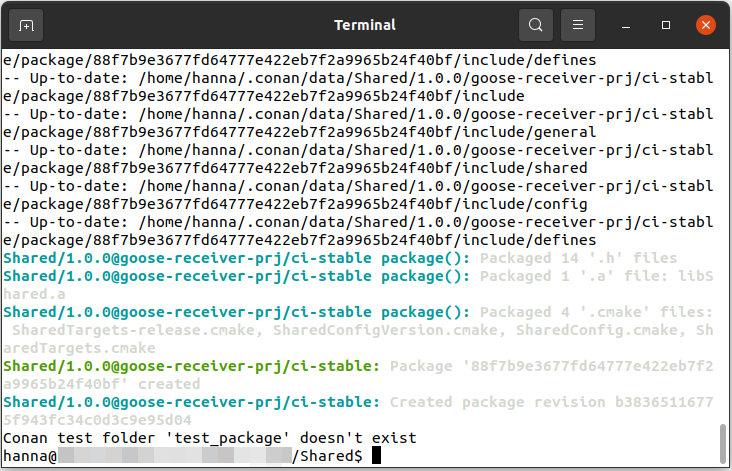
\includegraphics[width=0.8\linewidth]{SharedPackageBuildLog}
    \caption{Результаты сборки пакета Shared}
    \label{pic::manual::sharedPkgBuild}
\end{figure}

Переменная \lstinline{CUSTOM_CONAN_BUILD_TYPE} описывает тип сборки, возможные
значения и описание которых приведены в таблице~\ref{table:manual:buildTypes}.
Эти значения совпадают для Conan и CMake, который вызывается
Conan. Каждый из перечисленных вариантов преследует различные цели.
Так, например, вариант Release ориентирован на минимизацию времени исполнения кода,
тогда как MinSizeRel может пожертвовать скоростью работы в пользу меньшего
размера итогового файла.
В итоге каждый из приведенных типов сборки соответствует определенным наборам флагов
компилятора и в некоторых случаях компоновщика для достижения максимальной
эффективности.
Переопределить флаги можно в файле опций набора инструментов, который
используется CMake.

В результате сборки должен появиться вывод, аналогичный
рисунку~\ref{pic::manual::sharedPkgBuild}.

После успешной сборки вспомогательных пакетов необходимо произвести компиляцию
платформозависимого кода для операционной системы Linux. Это необходимо
сделать для проведения тестирования остальных пакетов на текущем компьютере.
Выполнение описанных ниже команд в терминале произведут необходимую сборку.
В результате будет получен вывод, аналогичный
рисунку~\ref{pic::manual::osalPkgBuild}.

\begin{lstlisting}
$ cd "$HOME/dvd"
$ export CI_COMMIT_TAG="1.0.0"
$ export CONAN_REMOTE_USER_OR_URL_SUFFIX="goose-receiver-prj"
$ cd OSAL
$ CUSTOM_CONAN_PROFILE=x86_64.gcc11.conf CUSTOM_CONAN_BUILD_TYPE=Release ./scripts/conan-run.py
\end{lstlisting}

\fixTableSectionSpace

\begin{figure}[ht]
    \centering
    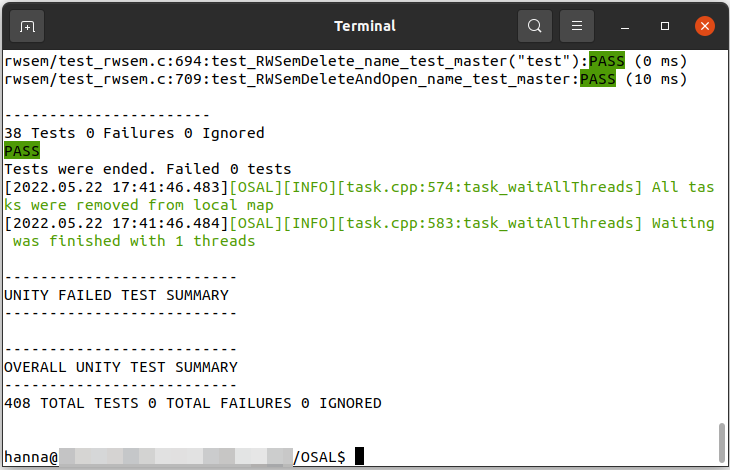
\includegraphics[width=0.8\linewidth]{OsalPackageBuildLog}
    \caption{Результаты сборки и тестирования пакета OSAL}
    \label{pic::manual::osalPkgBuild}
\end{figure}

\fixTableSectionSpace

\subsection{Автоматизированное тестирование}

Если посмотреть вывод скрипта сборки на рисунке~\ref{pic::manual::osalPkgBuild},
то можно увидеть результаты прохождения
тестирования под операционную систему Linux.
Отключение автоматического исполнения тестов можно произвести с помощью приведенной ниже
команды в терминале, из которого выполняется сборка.

\begin{lstlisting}
$ export GITLAB_CI=1
\end{lstlisting}

В результате выполнения этой команды последующие сборки из этого терминала
будут пропускать этап исполнения тестов.

Если по умолчанию запуск тестов не производится, то существует несколько
возможных вариантов:
\begin{itemize}
    \item происходит кросс-компиляция -- сборка под другую целевую архитектуру или операционную систему;
    \item отключено исполнение тестов описанным выше способом.
\end{itemize}

В первом случае ничего изменить не получится, поскольку запустить
тесты другой аппаратной или программной платформы без эмуляции не представляется
возможным.
Во втором же случае поведение можно вернуть на ожидаемое выполнением следующей
команды:

\begin{lstlisting}
$ export GITLAB_CI=
\end{lstlisting}

В результате в текущем терминале выполнение тестов после их сборки
будет возобновлено.

\subsection{Интеграция со средой разработки}

Для того, чтобы иметь возможность собирать проекты с помощью
интегрированной среды разработки и подтягивать необходимые
библиотеки из Conan, необходимо в настройки компилятора добавить
файл с настройками сборки и связывания из Conan и CMake.

Файл с опциями командной строки для компиляции исходных кодов имеет название
\lstinline!conan.ide.${CMAKE_SYSTEM_PROCESSOR}.include.opt!,
настройки компоновщика располагаются в
\lstinline!conan.ide.${CMAKE_SYSTEM_PROCESSOR}.link.opt!.
Содержимое директории \lstinline!conan.ide.out/ide/! создается путем вызова скрипта
сборки под необходимый целевой процессор и содержит описанные выше файлы.

Все пути приведены относительно корневой директории конкретного пакета, такой как
OSAL, Shared или GooseReceiver.
\lstinline!${CMAKE_SYSTEM_PROCESSOR}! является переменной CMake и
описывает имя процессора, под который будет производится сборка.
Обычно ее значение хранится в файле с настройками используемого набора инструментов
для CMake. Отличие данной переменной от значения, записанного в
\lstinline!${CMAKE_HOST_SYSTEM_PROCESSOR}!, приведет к выполнению
кросс-компиляции.

Для набора инструментов GCC добавление нескольких настроек компиляции делается с помощью
опции командной строки
\lstinline`@file.opt`, настроек связывания -- \lstinline`-Wl,-Tfile.opt`.
В обоих случаях приведен пример по добавлению файла \lstinline`file.opt`.
Вместо этого значения имени файла необходимо использовать тот,
который содержит настройки текущей целевой архитектуры и операционной
системы и располагается по указанному ранее пути. Принадлежность
к ним можно определить с помощью имени файла.
Расширение \lstinline{.include.opt} соответствует настройкам компиляции,
\lstinline{.link.opt} -- связывания.

Добавление настроек наборов инструментов конкретной среды разработки
обычно производится путем взаимодействия
с ее графическим интерфейсом. Обычно группы настроек компиляции не поддерживаются
как отдельная категория и представлена в разделе дополнительных или расширенных
опций с помощью возможности явного указания флагов, которые будут переданы
компилятору.
Набор настроек связывания обычно поддерживается графическими интерфейсами
в качестве конкретной опции, поскольку для корректной работы встраиваемых систем
их необходимо связывать с помощью специальных файлов с настройками различных секций
и доступной памяти.

В случае необходимости получения опций командной строки
для добавления файлов с настройками сборки и связывания
других наборов инструментов
обратитесь к руководству пользователя, которое предоставлено его разработчиками.
